% THIS DOCUMENT IS TAILORED TO REQUIREMENTS FOR SCIENTIFIC COMPUTING.  IT SHOULDN'T
% BE USED FOR NON-SCIENTIFIC COMPUTING PROJECTS
\documentclass[12pt]{article}

\usepackage{amsmath, mathtools}
\usepackage{amsfonts}
\usepackage{amssymb}
\usepackage{graphicx}
\usepackage{colortbl}
\usepackage{xr}
\usepackage{hyperref}
\usepackage{longtable}
\usepackage{xfrac}
\usepackage{tabularx}
\usepackage{float}
\usepackage{siunitx}
\usepackage{booktabs}
\usepackage{caption}
\usepackage{pdflscape}
\usepackage{afterpage}
\usepackage{hyperref}

\usepackage[round]{natbib}

%\usepackage{refcheck}

\hypersetup{
    bookmarks=true,         % show bookmarks bar?
      colorlinks=true,       % false: boxed links; true: colored links
    linkcolor=red,          % color of internal links (change box color with linkbordercolor)
    citecolor=green,        % color of links to bibliography
    filecolor=magenta,      % color of file links
    urlcolor=cyan           % color of external links
}

%% Comments

\usepackage{color}

\newif\ifcomments\commentstrue %displays comments
%\newif\ifcomments\commentsfalse %so that comments do not display

\ifcomments
\newcommand{\authornote}[3]{\textcolor{#1}{[#3 ---#2]}}
\newcommand{\todo}[1]{\textcolor{red}{[TODO: #1]}}
\else
\newcommand{\authornote}[3]{}
\newcommand{\todo}[1]{}
\fi

\newcommand{\wss}[1]{\authornote{blue}{SS}{#1}} 
\newcommand{\plt}[1]{\authornote{magenta}{TPLT}{#1}} %For explanation of the template
\newcommand{\an}[1]{\authornote{cyan}{Author}{#1}}

%% Common Parts

\newcommand{\progname}{ImgBeamer} % PUT YOUR PROGRAM NAME HERE
\newcommand{\authname}{Joachim de Fourestier} % AUTHOR NAMES                  

\usepackage{hyperref}
    \hypersetup{colorlinks=true, linkcolor=blue, citecolor=blue, filecolor=blue,
                urlcolor=blue, unicode=false}
    \urlstyle{same}
                                


% For easy change of table widths
\newcommand{\colZwidth}{1.0\textwidth}
\newcommand{\colAwidth}{0.13\textwidth}
\newcommand{\colBwidth}{0.82\textwidth}
\newcommand{\colCwidth}{0.1\textwidth}
\newcommand{\colDwidth}{0.05\textwidth}
\newcommand{\colEwidth}{0.8\textwidth}
\newcommand{\colFwidth}{0.17\textwidth}
\newcommand{\colGwidth}{0.5\textwidth}
\newcommand{\colHwidth}{0.28\textwidth}

% Used so that cross-references have a meaningful prefix
\newcounter{defnum} %Definition Number
\newcommand{\dthedefnum}{GD\thedefnum}
\newcommand{\dref}[1]{GD\ref{#1}}
\newcounter{datadefnum} %Datadefinition Number
\newcommand{\ddthedatadefnum}{DD\thedatadefnum}
\newcommand{\ddref}[1]{DD\ref{#1}}
\newcounter{theorynum} %Theory Number
\newcommand{\tthetheorynum}{T\thetheorynum}
\newcommand{\tref}[1]{T\ref{#1}}
\newcounter{tablenum} %Table Number
\newcommand{\tbthetablenum}{T\thetablenum}
\newcommand{\tbref}[1]{TB\ref{#1}}
\newcounter{assumpnum} %Assumption Number
\newcommand{\atheassumpnum}{P\theassumpnum}
\newcommand{\aref}[1]{A\ref{#1}}
\newcounter{goalnum} %Goal Number
\newcommand{\gthegoalnum}{P\thegoalnum}
\newcommand{\gsref}[1]{GS\ref{#1}}
\newcounter{instnum} %Instance Number
\newcommand{\itheinstnum}{IM\theinstnum}
\newcommand{\iref}[1]{IM\ref{#1}}
\newcounter{reqnum} %Requirement Number
\newcommand{\rthereqnum}{P\thereqnum}
\newcommand{\rref}[1]{R\ref{#1}}
\newcounter{nfrnum} %NFR Number
\newcommand{\rthenfrnum}{NFR\thenfrnum}
\newcommand{\nfrref}[1]{NFR\ref{#1}}
\newcounter{lcnum} %Likely change number
\newcommand{\lthelcnum}{LC\thelcnum}
\newcommand{\lcref}[1]{LC\ref{#1}}

\usepackage{fullpage}

\newcommand{\deftheory}[9][Not Applicable]
{
\newpage
\noindent \rule{\textwidth}{0.5mm}

\paragraph{RefName: } \textbf{#2} \phantomsection 
\label{#2}

\paragraph{Label:} #3

\noindent \rule{\textwidth}{0.5mm}

\paragraph{Equation:}

#4

\paragraph{Description:}

#5

\paragraph{Notes:}

#6

\paragraph{Source:}

#7

\paragraph{Ref.\ By:}

#8

\paragraph{Preconditions for \hyperref[#2]{#2}:}
\label{#2_precond}

#9

\paragraph{Derivation for \hyperref[#2]{#2}:}
\label{#2_deriv}

#1

\noindent \rule{\textwidth}{0.5mm}

}

\begin{document}

\title{Software Requirements Specification for \progname: SEM Image Formation} 
\author{\authname}
\date{\today}
	
\maketitle

~\newpage

\pagenumbering{roman}

\tableofcontents

~\newpage

\section*{Revision History}

\begin{tabularx}{\textwidth}{p{3cm}p{2cm}X}
\toprule {\bf Date} & {\bf Version} & {\bf Notes}\\
\midrule
2023/02/02 & 1.0 & First version\\
Date 2 & 1.1 & Notes\\
\bottomrule
\end{tabularx}

~\newpage

\section{Reference Material}

This section records information for easy reference.

\subsection{Table of Units}

Throughout this document SI (Syst\`{e}me International d'Unit\'{e}s) is employed
as the unit system.  In addition to the basic units, several derived units are
used as described below.  For each unit, the symbol is given followed by a
description of the unit and the SI name.
~\newline

\renewcommand{\arraystretch}{1.2}
%\begin{table}[ht]
  \noindent \begin{tabular}{l l l} 
    \toprule		
    \textbf{symbol} & \textbf{unit} & \textbf{SI}\\
    \midrule 
    \si{\metre} & length & metre\\
    \si{\second} & time & second\\
    \si{Pa} & pressure & pascal\\
    \si{J} & energy & joule\\
    \si{K} & temperature & kelvin\\
    \si{mol} & substance & mole\\
    \bottomrule
  \end{tabular}
  %	\caption{SI Units}
%\end{table}
~\newline
 
~\newline
Additional units used:
~\newline

%\begin{table}[ht]
  \noindent \begin{tabular}{l l l} 
    \toprule		
    \textbf{symbol} & \textbf{unit} & \textbf{name}\\
    \midrule
    px & pixel & picture element ?\\
    \si{\nm} & length & nanometre (\num{d-9} m)\\
    \si{\um} & length & micrometre (\num{d-6} m)\\
    \bottomrule
  \end{tabular}
  %	\caption{SI Units}
%\end{table}

\subsection{Table of Symbols}

The table that follows summarizes the symbols used in this document along with
their units.  The choice of symbols was made to be consistent with the heat
transfer literature and with existing documentation for solar water heating
systems.  The symbols are listed in alphabetical order.

\renewcommand{\arraystretch}{1.2}
%\noindent \begin{tabularx}{1.0\textwidth}{l l X}
\noindent \begin{longtable*}{l l p{12cm}} \toprule
\textbf{symbol} & \textbf{unit} & \textbf{description}\\
\midrule 
$d_p$ & \si[per-mode=symbol] {\nm} & probe diameter (size)\\
$d_i$ & \si[per-mode=symbol] {\nm} & probe step size in image space\\
$d_o$ & \si[per-mode=symbol] {\nm} & probe step size in object space\\
$I_{n\times m}$ & 8-bit gray level & Image intensity matrix that has $n$ rows and $m$ columns.\\
$M_{n\times m}$ & boolean & Mask / stencil matrix that has $n$ rows and $m$ columns.\\
$R_{n\times m}$ & 8-bit gray level & Resulting image intensity matrix that has $n$ rows and $m$ columns.\\
\bottomrule
\end{longtable*}

\subsection{Abbreviations and Acronyms}

\renewcommand{\arraystretch}{1.2}
\begin{tabular}{l l} 
  \toprule		
  \textbf{symbol} & \textbf{description}\\
  \midrule 
  A & Assumption\\
  DD & Data Definition\\
  GD & General Definition\\
  GS & Goal Statement\\
  IM & Instance Model\\
  LC & Likely Change\\
  PS & Physical System Description\\
  R & Requirement\\
  SRS & Software Requirements Specification\\
  TM & Theoretical Model\\
  2D & two-dimensional\\
  3D & three-dimensional\\
  BSE & Backscattered Electron\\
  CCD & Charge Coupled Device\\
  EM & Electron Microscopy\\
  FOV & Field of View\\
  LM & Light Microscopy\\
  ROI & Region of Interest\\
  SEM & Scanning Electron Microscope\\
  SE & Secondary Electron\\
  \progname{} & SEM image formation demo tool\\
  \bottomrule
\end{tabular}\\

\pagenumbering{arabic}

\section{Introduction}

Images formed by Scanning Electron Microscope (SEM) are created using a 
specific process where the image quality can be greatly influenced by the 
imaging parameters given by the user, aside from any inherent electron 
optics limitation of a given instrument. The motivation of this project is 
to be able visualize qualitatively the influence of the spot profile 
(shape and size) and the rastering parameters (such as pixel size). Since the 
quality of an image is very often evaluated subjectively by an experienced 
microscope user, the idea behind this software is provide a way to show 
that adjusting the imaging parameters could lead to a loss of information 
or misinterpretation. Is is also to prove or disprove if there is a "rule 
of thumb" for the optimal spot-to-pixel size ratio.

\subsection{Purpose of Document}

This document serves as the software specification. The details of the 
requirements, limitations, definitions, models to be used are laid explicitly 
within this document.

\subsection{Scope of Requirements} 

The scope of the requirements of this software is restricted to only the image 
formation process used in SEMs, more specifically the image processing from 
signal to an image or visual representions. It does not cover election-sample 
interactions or CCD (charge coupled device) detector voltage to signal value 
conversion. See the assumptions section (Section~\ref{sec_assumpt}) for further 
details.

\subsection{Characteristics of Intended Reader} \label{sec_IntendedReader}

The intended reader of this document should have a basic understanding of 
electron-optics concepts used in an SEM. This can be equated to standard level 
two university physics (optics, electricity, magnetism, thermodynamics and 
modern physics) along with a standard undergraduate course related to materials 
characterization (concepts such as backscattered electrons, mean free path, and 
electron density). The reader should have a basic understanding of two-dimensional 
image processing techniques and level one university linear algebra (matrices).

\subsection{Organization of Document}

This document contains an introduction to the software and its goals. It is 
meant to be a reference document to the readers and is based on a SRS template from \citet{SmithAndLai2005, SmithEtAl2007}. The document include a 
description of the scope, a detailed list of the terminology, definitions, and 
models used, as well as a more specific and detailed description of the problem 
and its solutions. This document also defines the requirements, as well as the  
likely changes and traceability details.

\section{General System Description}

This section provides general information about the system.  It identifies the
interfaces between the system and its environment, describes the user
characteristics and lists the system constraints.

\plt{The purpose of this section is to provide general information about the
  system so the specific requirements in the next section will be easier to
  understand. The general system description section is designed to be
  changeable independent of changes to the functional requirements documented in
  the specific system description. The general system description provides a
  context for a family of related models.  The general description can stay the
  same, while specific details are changed between family members.}

\subsection{System Context}

\plt{Your system context will include a figure that shows the abstract view of
  the software.  Often in a scientific context, the program can be viewed
  abstractly following the design pattern of Inputs $\rightarrow$ Calculations
  $\rightarrow$ Outputs.  The system context will therefore often follow this
  pattern.  The user provides inputs, the system does the calculations, and then
  provides the outputs to the user.  The figure should not show all of the
  inputs, just an abstract view of the main categories of inputs (like material
  properties, geometry, etc.).  Likewise, the outputs should be presented from
  an abstract point of view.  In some cases the diagram will show other external
  entities, besides the user.  For instance, when the software product is a
  library, the user will be another software program, not an actual end user.
  If there are system constraints that the software must work with external
  libraries, these libraries can also be shown on the System Context diagram.
  They should only be named with a specific library name if this is required by
  the system constraint.}

\begin{figure}[h!]
\begin{center}
 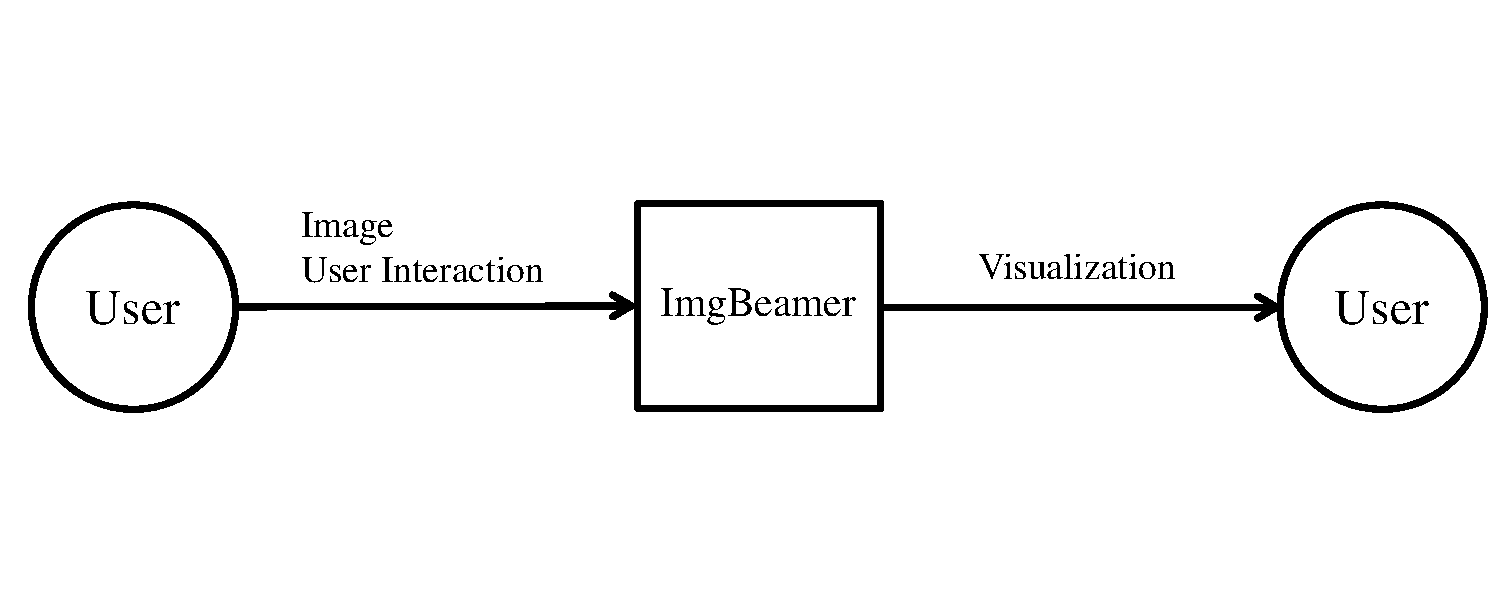
\includegraphics[width=0.6\textwidth]{SystemContextFigure}
\caption{System Context}
\label{Fig_SystemContext} 
\end{center}
\end{figure}

\plt{For each of the entities in the system context diagram its responsibilities
  should be listed.  Whenever possible the system should check for data quality,
  but for some cases the user will need to assume that responsibility.  The list
  of responsibilites should be about the inputs and outputs only, and they
  should be abstract.  Details should not be presented here.  However, the
  information should not be so abstract as to just say ``inputs'' and
  ``outputs''.  A summarizing phrase can be used to characterize the inputs.
  For instance, saying ``material properties'' provides some information, but it
  stays away from the detail of listing every required properties.}

\begin{itemize}
\item User Responsibilities:
\begin{itemize}
\item 
\end{itemize}
\item \progname{} Responsibilities:
\begin{itemize}
\item Detect data type mismatch, such as a string of characters instead of a
  floating point number
\item 
\end{itemize}
\end{itemize}

\subsection{User Characteristics} \label{SecUserCharacteristics}

The \progname{} software end user is anyone that has used an SEM or is learning about them. This ranges from a university undergraduate science student in which their curriculum includes electron microscopy (EM), to experienced SEM operators or even to experts in the field of EM. The software end users also includes those described in Section~\ref{sec_IntendedReader} (intender readers of this document). That said, image processing nor linear algebra knowledge is not required. 

\subsection{System Constraints}

\plt{System constraints differ from other type of requirements because they
  limit the developers' options in the system design and they identify how the
  eventual system must fit into the world. This is the only place in the SRS
  where design decisions can be specified.  That is, the quality requirement for
  abstraction is relaxed here.  However, system constraints should only be
  included if they are truly required.}

\section{Specific System Description}

This section first presents the problem description, which gives a high-level
view of the problem to be solved.  This is followed by the solution characteristics
specification, which presents the assumptions, theories, definitions and finally
the instance models.

\subsection{Problem Description} \label{Sec_pd}

\progname{} is intended to help visualize and understand the influence of the 
spot profile and pixel size. It should be able to help determine the optimal 
spot-to-pixel-size ratio.

\subsubsection{Terminology and Definitions}

This subsection provides a list of terms that are used in the subsequent
sections and their meaning, with the purpose of reducing ambiguity and making it
easier to correctly understand the requirements:

\begin{center}
    \noindent
    \begin{longtable}{p{4.25cm} p{11.25cm}} 
        \toprule
        \textbf{Terminology} & \textbf{Definition}\\
        \midrule
        Backscattered Electron & An electron that is elastically scattered backwards to the initial direction of travel as a result of electron-sample interactions between the beam and the sample. \\
        
        Beam & The continuous focused stream of electrons accelerated at high speeds down the column of an electron microscope. \\

        Bit Depth & It is the range of the value (intensity or color) of a pixel. Specifically, it is the maximum number of bits used to represent said value. \\
        
        Brightness & The intensity value (or perceived luminance for colours) of a signal, point (or pixel), or area within an image. \\
        
        Contrast & The difference or distinguisable quality of an intensity (or colour) or brightness value of a point (or pixel) from another point in an image.\\
        
        Electron-Sample\newline Interactions & The interactions as a result of electrons from the beam hitting the sample surface leading to an electron collision cascade. This in produces various emissions such as x-rays, BSEs, and SEs. \\
        
        Electron Microscopy & The practice of microscopes that specifically use electrons as the source of illumination to produce an image or signal.  \\
        
        Exact-sampling & The sampling size or rate that matches the specificity of the targeted resolution. In the context of this document, this is when the size of the probe that matches the size of the pixel. \\
        
        Field of View & The observable or visible extent given by the microscope and varies with magnification. \\
        
        Ground Truth & The data or information that is considered as the source or reference standard of truth. \\
        
        Image & A representation of visual information that can be represented by 2D matrix where each cell represents a pixel with a specific value (representative of intensity or colour). -- \\
        
        Image Quality & The perceived clarity, amount of information or detail representative of reality that is contained within an image. \\
        
        Image Resolution & The size dimensions (width and height) of an image. Typically, it is defined in pixels. \\
        
        Interaction Volume & The volume within the sample in which there are electron-sample interactions caused by the beam coming into contact with the surface of the sample. \\
        
        Light Microscopy & The practice of microscopes that specifically use light as the source of illumination to produce an image or signal. \\

        Mean Free Path & The average distance within a system that a particle can travel before it collides with other particles.\\
        
        Nyquist Limit & More formally known as the "Nyquist-Shannon" sampling limit is the minimum sampling rate at which all the essential information is captured when discretizing a continous signal, resulting in little to no distortions. \\
        
        Over-sampling & This is a sampling rate or size that is too large where the specificity or origin of the information is lost. This generally results in increased confidence, but at a loss of precision.\\
        
        Pixel Size & The size or dimensions of one cell within a raster grid. \\
        
        Probe & Generally interchangeable with "beam". Contextually within this document, it is the final part of the beam that comes into contact with the surface of the sample (being analysed within the microscope) forming a "spot" with a targeted size and shape. \\
        
        Raster Grid & A scanning pattern with a defined and repeated cell size. \\
        
        Region of Interest & A defined 2D area in both position, size, and shape on a sample. \\
        
        Resolution & As defined by the Rayleigh criterion, it is the minimum distance by which two points or features can be distinguished. \\
        
        Secondary Electron & An electron that emitted from the sample as a result of inelastic electron-sample interactions between the beam and the sample. These can be weakly bounded valence electrons or conduction band electrons. \\
        
        Signal-to-Noise Ratio & The amount of information (signal) considered useful or representative of reality versus the amount of noise. \\
        
        Spot Shape & The overall shape of the spot or probe, whether is it a perfect circle or elongated ellipse, or even a halo or ring. \\
        
        Spot Size & The overall diameter or average feret/caliper diameter of the probe. \\
        
        Step Size & The length or distance of a "pixel" by which the probe is moved or deflected to when raster scanning the surface of a sample. \\
        
        Subregion & A region or area contained within the current FOV. \\

        Under-sampling & This is a sampling rate or size that is too small where the specificity or origin of the information is more restricted. This generally results in increased precision, but at a loss of confidence, or even accuracy. \\
        \bottomrule
    \end{longtable} 
\end{center}

\subsubsection{Physical System Description} \label{sec_phySystDescrip}

The physical system of \progname{}, as shown in Figure \ref{fig_ebeam} and \ref{fig_sampling},
includes the following elements:

\begin{itemize}

\item[PS1:] The sample that is being imaged or studied.

\item[PS2:] An SEM which includes a BSE and/or SE detector. The electron beam interacts with the sample surface in high-vacuum producing various signals.

\end{itemize}

\setlength{\belowcaptionskip}{-30pt}
\begin{figure}[h!]
\begin{center}
{
 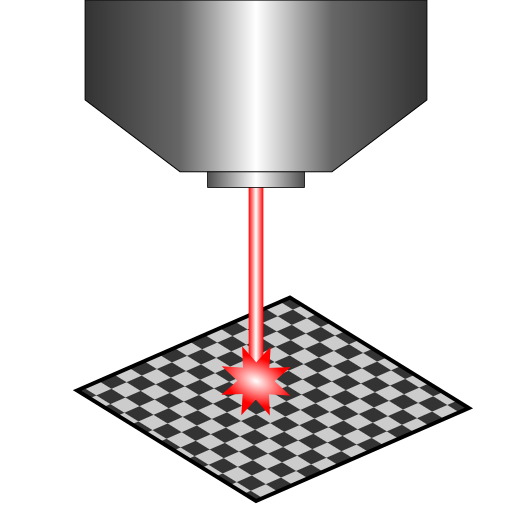
\includegraphics[width=0.3\textwidth]{figures/e_beam.png}
}
\caption{\label{fig_ebeam} Schematic drawing of an electron beam hitting the sample surface within an SEM chamber. (Image from: \url{https://github.com/joedf/ImgBeamer})}
\end{center}
\end{figure}

\begin{figure}[h!]
\begin{center}
{
 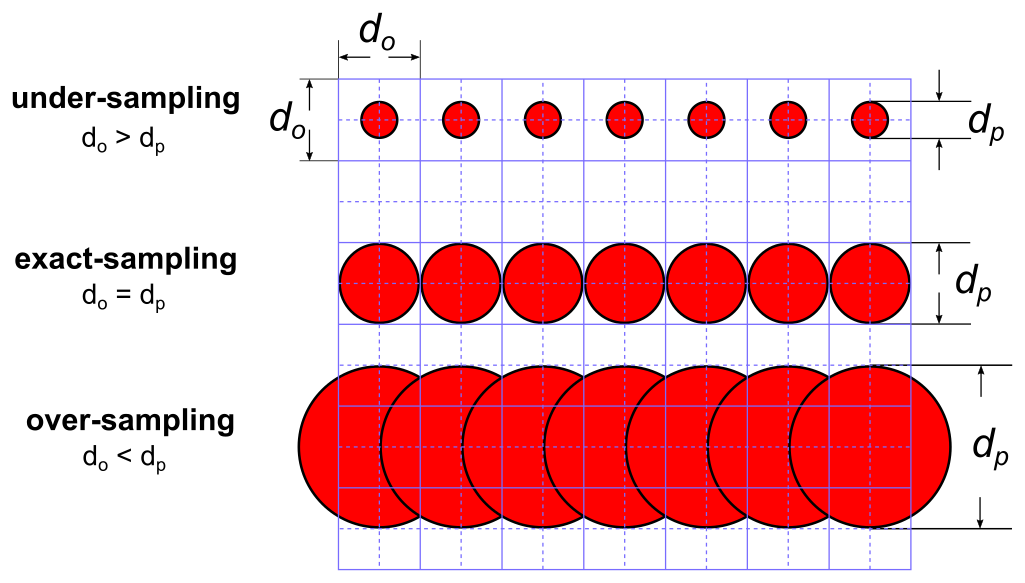
\includegraphics[width=0.8\textwidth]{figures/sampling.png}
}
\caption{\label{fig_sampling} Schematic of the three sampling scenarios (under-sampling, exact-sampling, and over-sampling) and a visual representation of the pixel grid, $d_p$, and $d_o$. The dashed lines are to help visualize the center of each pixel cell. Adapted from \citet{lifshin_improving_2014}}
\end{center}
\end{figure}

\subsubsection{Goal Statements}

\noindent Given an image, the goal statements are:

\begin{itemize}

\item[GS\refstepcounter{goalnum}\thegoalnum \label{G_easeofuse}:] {
A user-friendly straight forward tool to load and reprocess an image with options following the SEM image formation process.
}

\item[GS\refstepcounter{goalnum}\thegoalnum \label{G_metric}:] {
Provide a quantitative metric of relative image quality of the resulting image created from the given parameters and input image (as ground truth).
}

\item[GS\refstepcounter{goalnum}\thegoalnum \label{G_visualize}:] {
The ability to visualize and export the reprocessed images.
}

\end{itemize}

\subsection{Solution Characteristics Specification}

This section provides the assumptions, instance models, theoretical models, general definitions, and the data constraints. The information specfied in this section is intended to reduce ambiguities and reduce the problem into clear logical or mathematical terms.

\begin{figure}[H]
  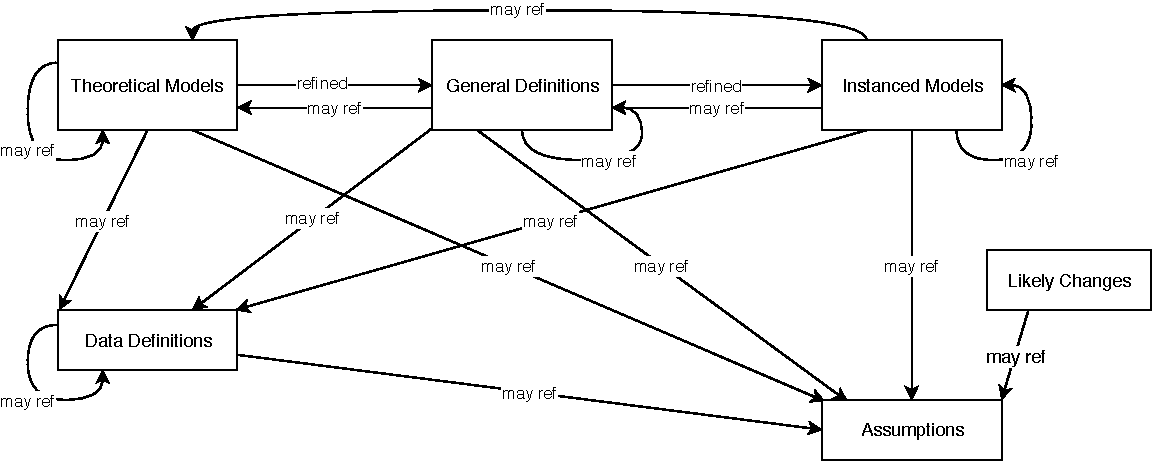
\includegraphics[scale=0.9]{RelationsBetweenTM_GD_IM_DD_A.pdf}
\end{figure}

The instance models that govern \progname{} are presented in
Subsection~\ref{sec_instance}.  The information to understand the meaning of the
instance models and their derivation is also presented, so that the instance
models can be verified.

\subsubsection{Assumptions} \label{sec_assumpt}

This section simplifies the original problem and helps in developing the
theoretical model by filling in the missing information for the physical
system. The numbers given in the square brackets refer to the theoretical model
[TM], general definition [GD], data definition [DD], instance model [IM], or
likely change [LC], in which the respective assumption is used.

\begin{itemize}

\item[A\refstepcounter{assumpnum}\theassumpnum \label{A_sample}:] The sample 
surface is solid, flat (meaning no topography), orthogonal to the beam, and 
conductive (meaning no charge build up from electrons). The material is made of 
atoms with atomic numbers greater than 3 (lithium).

\item[A\refstepcounter{assumpnum}\theassumpnum \label{A_beam}:] The electron 
beam is ideal: meaning stable and colliminated meaning all the electrons are 
traveling parallel to each other down towards the sample surface within high 
vacuum (optimal mean free path). The beam intensity or current is considered 
uniform throughout the beam.

\item[A\refstepcounter{assumpnum}\theassumpnum \label{A_inputImage}:] The input 
image of the sample is considered to have infinite resolution representive of reality: ground truth.

\item[A\refstepcounter{assumpnum}\theassumpnum \label{A_yield}:] The BSEs and SEs
yields are high enough to produce enough signal and noise is low, meaning optimal SNR.

\item[A\refstepcounter{assumpnum}\theassumpnum \label{A_environment}:] The SEM 
is within a climate controlled (temperature and humidity) and low vibration room.

\item[A\refstepcounter{assumpnum}\theassumpnum \label{A_reality}:] The image 
produced by the SEM as the electron raster scan the sample surface is an 
approximate representation of reality.

\end{itemize}

\subsubsection{Theoretical Models}\label{sec_theoretical}

This section focuses on the general equations and laws that \progname{} is based
on.
~\newline

\noindent
\begin{minipage}{\textwidth}
\renewcommand*{\arraystretch}{1.5}
\begin{tabular}{| p{\colAwidth} | p{\colBwidth}|}
  \hline
  \rowcolor[gray]{0.9}
  Number& TM\refstepcounter{theorynum}\thetheorynum \label{T_label1}\\
  \hline
  Label& \bf Mean Free Path\\
  \hline
  Equation &
    $\lambda = \frac{RT}{\sqrt{2}\pi d^{2}N_AP}$ \\[3pt]
  \hline
  Description
    & $\lambda$ is the mean free path (\si{m}) \\
    & $R$ is the universal gas constant = $8.3145$ \si{J/mol.K} \\
    & $T$ is the temperature (\si{K}) \\
    & $d$ is the molecular diameter (\si{m}) \\
    & $P$ is the pressure (\si{Pa}) \\
    & $N_A$ is Avogadro's number = $6.0221 \times 10^{23}$ \si{\per\mol} \\
  \hline
  Notes & -- \\
  \hline
  Sources& \url{http://hyperphysics.phy-astr.gsu.edu/hbase/Kinetic/menfre.html} \\
  \hline
  Ref.\ By & \aref{A_beam} \\
  \hline
\end{tabular}
\end{minipage}\\

\noindent
\begin{minipage}{\textwidth}
\renewcommand*{\arraystretch}{1.5}
\begin{tabular}{| p{\colAwidth} | p{\colBwidth}|}
  \hline
  \rowcolor[gray]{0.9}
  Number& TM\refstepcounter{theorynum}\thetheorynum \label{T_label2}\\
  \hline
  Label& \bf Contrast\\
  \hline
  Equation & $C_{tr} = (S_{max} - S_{min}) / S_{max}$ \\
  \hline
  Description & -- \\
  \hline
  Notes & -- \\
  \hline
  Sources& \cite{goldstein_image_2018} \\
  \hline
  Ref.\ By & -- \\
  \hline
\end{tabular}
\end{minipage}\\

~\newline

\subsubsection{General Definitions}\label{sec_gendef}

\plt{General Definitions (GDs) are a refinement of one or more TMs, and/or of
  other GDs.  The GDs are less abstract than the TMs.  Generally the reduction
  in abstraction is possible through invoking (using/referencing) Assumptions.
  For instance, the TM could be Newton's Law of Cooling stated abstracting.  The
  GD could take the general law and apply it to get a 1D equation.}

This section collects the laws and equations that will be used in building the
instance models.

\plt{Some projects may not have any content for this section, but the section
  heading should be kept.}  \plt{Modify the examples below for your problem, and
  add additional definitions as appropriate.}

~\newline

\noindent
\begin{minipage}{\textwidth}
\renewcommand*{\arraystretch}{1.5}
\begin{tabular}{| p{\colAwidth} | p{\colBwidth}|}
\hline
\rowcolor[gray]{0.9}
Number& GD\refstepcounter{defnum}\thedefnum \label{NL}\\
\hline
Label &\bf Newton's law of cooling \\
\hline
% Units&$MLt^{-3}T^0$\\
% \hline
SI Units&\si{\watt\per\square\metre}\\
\hline
Equation&$ q(t) = h \Delta T(t)$  \\
\hline
Description &
Newton's law of cooling describes convective cooling from a surface.  The law is
stated as: the rate of heat loss from a body is proportional to the difference
in temperatures between the body and its surroundings.
\\
& $q(t)$ is the thermal flux (\si{\watt\per\square\metre}).\\
& $h$ is the heat transfer coefficient, assumed independent of $T$ (\aref{A_hcoeff})
	(\si{\watt\per\square\metre\per\celsius}).\\
&$\Delta T(t)$= $T(t) - T_{\text{env}}(t)$ is the time-dependent thermal gradient
between the environment and the object (\si{\celsius}).
\\
\hline
  Source & Citation here \\
  \hline
  Ref.\ By & \ddref{FluxCoil}, \ddref{FluxPCM}\\
  \hline
\end{tabular}
\end{minipage}\\

\subsubsection*{Detailed derivation of simplified rate of change of temperature}

\plt{This may be necessary when the necessary information does not fit in the
  description field.}
\plt{Derivations are important for justifying a given GD.  You want it to be
  clear where the equation came from.}

\subsubsection{Data Definitions}\label{sec_datadef}

\plt{The Data Definitions are definitions of symbols and equations that are
  given for the problem.  They are not derived; they are simply used by other
  models.  For instance, if a problem depends on density, there may be a data
  definition for the equation defining density.  The DDs are given information
  that you can use in your other modules.}

\plt{All Data Definitions should be used (referenced) by at least one other
  model.}

This section collects and defines all the data needed to build the instance
models. The dimension of each quantity is also given.  \plt{Modify the examples
  below for your problem, and add additional definitions as appropriate.}

~\newline

\noindent
\begin{minipage}{\textwidth}
\renewcommand*{\arraystretch}{1.5}
\begin{tabular}{| p{\colAwidth} | p{\colBwidth}|}
\hline
\rowcolor[gray]{0.9}
Number& DD\refstepcounter{datadefnum}\thedatadefnum \label{FluxCoil}\\
\hline
Label& \bf Heat flux out of coil\\
\hline
Symbol &$q_C$\\
\hline
% Units& $Mt^{-3}$\\
% \hline
  SI Units & \si{\watt\per\square\metre}\\
  \hline
  Equation&$q_C(t) = h_C (T_C - T_W(t))$, over area $A_C$\\
  \hline
  Description & 
                $T_C$ is the temperature of the coil (\si{\celsius}).  $T_W$ is the temperature of the water (\si{\celsius}).  
                The heat flux out of the coil, $q_C$ (\si{\watt\per\square\metre}), is found by
                assuming that Newton's Law 
                of Cooling applies (\aref{A_Newt_coil}).  This law (\dref{NL}) is used on the surface of
                the coil, which has area $A_C$ (\si{\square\metre}) and heat 
                transfer coefficient $h_C$
                (\si{\watt\per\square\metre\per\celsius}).  This equation
                assumes that the temperature of the coil is constant over time (\aref{A_tcoil}) and that it does not vary along the length
                of the coil (\aref{A_tlcoil}).
  \\
  \hline
  Sources& Citation here \\
  \hline
  Ref.\ By & \iref{ewat}\\
  \hline
\end{tabular}
\end{minipage}\\

\subsubsection{Data Types}\label{sec_datatypes}

\plt{This section is optional.  In many scientific computing programs it isn't
  necessary, since the inputs and outpus are straightforward types, like reals,
  integers, and sequences of reals and integers.  However, for some problems it
  is very helpful to capture the type information.}

\plt{The data types are not derived; they are simply stated and used by other
  models.}

\plt{All data types must be used by at least one of the models.}

\plt{For the mathematical notation for expressing types, the recommendation is
  to use the notation of~\citet{HoffmanAndStrooper1995}.}

This section collects and defines all the data types needed to document the
models. \plt{Modify the examples below for your problem, and add additional
  definitions as appropriate.}

~\newline

\noindent
\begin{minipage}{\textwidth}
\renewcommand*{\arraystretch}{1.5}
\begin{tabular}{| p{\colAwidth} | p{\colBwidth}|}
  \hline
  \rowcolor[gray]{0.9}
  Type Name & Name for Type\\
  \hline
  Type Def & mathematical definition of the type\\
  \hline
  Description & description here
  \\
  \hline
  Sources & Citation here, if the type is borrowed from another source\\
  \hline
\end{tabular}
\end{minipage}\\

\subsubsection{Instance Models} \label{sec_instance}    

This section transforms the problem defined in Section~\ref{Sec_pd} into 
one which is expressed in mathematical terms. It uses concrete symbols defined 
in Section~\ref{sec_datadef} to replace the abstract symbols in the models 
identified in Sections~\ref{sec_theoretical} and~\ref{sec_gendef}.

The goal of reprocessing an image \gsref{G_easeofuse} will be solved by \iref{IM_bitblt}. The goal of providing an image quality metric will be solved by \iref{IM_imageMetric}.  

~\newline

%Instance Model 1

\noindent
\begin{minipage}{\textwidth}
\renewcommand*{\arraystretch}{1.5}
\begin{tabular}{| p{\colAwidth} | p{\colBwidth}|}
  \hline
  \rowcolor[gray]{0.9}
  Number& IM\refstepcounter{instnum}\theinstnum \label{IM_bitblt}\\
  \hline
  Label& \bf Bit blit (as known as Bit Block Transfer) \\
  \hline
  Input& an image $I_{n \times m}$ and a mask $M_{n \times m}$\\
  \hline
  Output& reprocessed image $R_{n \times m}$ \\
  \hline
  Description
  & Given an image and mask (or stencil), a boolean operation is performed iteratively
  on each cell of the image matrix, based on the corresponding cell value found in the mask
  matrix at row $i$ and column $j$.\\
  
  & If the mask cell value (at $i$, $j$) is true (or any non-zero value), the corresponding image
  cell value is transfered/kept in the resulting/destination matrix.\\

  & Otherwise, if the corresponding
  matrix cell (at $i$, $j$) is false (zero), then no value is transfered, and zero will inserted
  at $i$, $j$ in the destination image matrix. \\
  \hline
  Sources& \url{https://en.wikipedia.org/wiki/Bit\_blit} \\
  \hline
  Ref.\ By & \rref{R_resultImage} \\
  \hline
\end{tabular}
\end{minipage}\\

%Instance Model 2

\noindent
\begin{minipage}{\textwidth}
\renewcommand*{\arraystretch}{1.5}
\begin{tabular}{| p{\colAwidth} | p{\colBwidth}|}
  \hline
  \rowcolor[gray]{0.9}
  Number& IM\refstepcounter{instnum}\theinstnum \label{IM_imageMetric}\\
  \hline
  Label& \bf Image quality metric / evaluation \\
  \hline
  Input& a image $I_{n \times m}$ serving as ground truth and the image $R_{n \times m}$ to compare\\
  \hline
  Output& a positive ratio value ranging from $0$ to $1.00$.\\
  \hline
  Description
  & Given the original image (ground truth) and a reprocessed image, a 
  metric must be calculated to express image similarity where $1.00$ means
  a perfect match and $0.00$ means absolutely no correlation or similarity found.\\

  & If the images do no match in size, the smaller (or larger?) image shall be scaled to match.\\

  & The values do not need to be absolutely quantitative. They only need to 
  be relatively comparable when only changing $d_p$ or the spot shape.\\
  \hline
  Sources& \\
  \hline
  Ref.\ By & \rref{R_imageMetric}, \nfrref{NFR_Usability} \\
  \hline
\end{tabular}
\end{minipage}\\

%~\newline

\subsubsection{Input Data Constraints} \label{sec_DataConstraints}    

Table~\ref{TblInputVar} shows the data constraints on the input output
variables.  The column for physical constraints gives the physical limitations
on the range of values that can be taken by the variable.  The column for
software constraints restricts the range of inputs to reasonable values.  The
software constraints will be helpful in the design stage for picking suitable
algorithms.  The constraints are conservative, to give the user of the model the
flexibility to experiment with unusual situations.  The column of typical values
is intended to provide a feel for a common scenario.  The uncertainty column
provides an estimate of the confidence with which the physical quantities can be
measured.  This information would be part of the input if one were performing an
uncertainty quantification exercise.

The specification parameters in Table~\ref{TblInputVar} are listed in
Table~\ref{TblSpecParams}.

\begin{table}[!h]
  \caption{Input Variables} \label{TblInputVar}
  \renewcommand{\arraystretch}{1.2}
\noindent \begin{longtable*}{l l l l c} 
  \toprule
  \textbf{Var} & \textbf{Physical Constraints} & \textbf{Software Constraints} &
                             \textbf{Typical Value} & \textbf{Uncertainty}\\
  \midrule 
  $L$ & $L > 0$ & $L_{\text{min}} \leq L \leq L_{\text{max}}$ & 1.5 \si[per-mode=symbol] {\metre} & 10\%
  \\
  \bottomrule
\end{longtable*}
\end{table}

\noindent 
\begin{description}
\item[(*)] \plt{you might need to add some notes or clarifications}
\end{description}

\begin{table}[!h]
\caption{Specification Parameter Values} \label{TblSpecParams}
\renewcommand{\arraystretch}{1.2}
\noindent \begin{longtable*}{l l} 
  \toprule
  \textbf{Var} & \textbf{Value} \\
  \midrule 
  $L_\text{min}$ & 0.1 \si{\metre}\\
  \bottomrule
\end{longtable*}
\end{table}

\subsubsection{Properties of a Correct Solution} \label{sec_CorrectSolution}

\noindent
A correct solution must exhibit \plt{fill in the details}.  \plt{These
  properties are in addition to the stated requirements.  There is no need to
  repeat the requirements here.  These additional properties may not exist for
  every problem.  Examples include conservation laws (like conservation of
  energy or mass) and known constraints on outputs, which are usually summarized
  in tabular form.  A sample table is shown in Table~\ref{TblOutputVar}}

\begin{table}[!h]
\caption{Output Variables} \label{TblOutputVar}
\renewcommand{\arraystretch}{1.2}
\noindent \begin{longtable*}{l l} 
  \toprule
  \textbf{Var} & \textbf{Physical Constraints} \\
  \midrule 
  $T_W$ & $T_\text{init} \leq T_W \leq T_C$ (by~\aref{A_charge})
  \\
  \bottomrule
\end{longtable*}
\end{table}

\plt{This section is not for test cases or techniques for verification and
  validation.  Those topics will be addressed in the Verification and Validation
  plan.}

\newpage
\section{Requirements}

This section provides the functional requirements, the business tasks that the
software is expected to complete, and the nonfunctional requirements, the
qualities that the software is expected to exhibit.

\subsection{Functional Requirements}

\noindent \begin{itemize}

\item[R\refstepcounter{reqnum}\thereqnum \label{R_Inputs}:] Accept an input 
image in the following formats:

  \noindent \begin{itemize}
    \item PNG (Portable Net Graphics)
    \item JPG (Joint Photographic Experts Group)
    \item BMP (Bitmap)
    \item preloaded example images
  \end{itemize}

\item[R\refstepcounter{reqnum}\thereqnum \label{R_userSpotProfile}:] Accept user 
input of the size and shape of the spot profile and ensure that all its defining 
values are positive real numbers.

\item[R\refstepcounter{reqnum}\thereqnum \label{R_userPixelSize}:] Accept user 
input of pixel size and ensure it is a positive real number.

\item[R\refstepcounter{reqnum}\thereqnum \label{R_subregion}:] Accept user
input to specify a subregion (FOV) for processing.

\item[R\refstepcounter{reqnum}\thereqnum \label{R_spotLayout}:] Display a 
representative spot layout used for processing the image.

\item[R\refstepcounter{reqnum}\thereqnum \label{R_resultImage}:] Reprocess 
(using \iref{IM_bitblt}) and display the resulting image to the user.

\item[R\refstepcounter{reqnum}\thereqnum \label{R_imageMetric}:] Calculate and 
display an image quality metric (according to \iref{IM_imageMetric}) to the user.

\end{itemize}

\subsection{Nonfunctional Requirements}

The key nonfunctional requirements of this software are accuracy, usability, 
maintainability, and portability. These are listed below in detail:

\noindent \begin{itemize}

\item[NFR\refstepcounter{nfrnum}\thenfrnum \label{NFR_Accuracy}:]
  \textbf{Accuracy} The images produced should be not manipulated to produce 
  results that subjectively represent the opinions of the author(s) or 
  developer(s). Thus, the software should transparently follow the 
  specifications and be verifiable by an expert in field. The trends in image 
  quality metric are more important the metric values themselves.

\item[NFR\refstepcounter{nfrnum}\thenfrnum \label{NFR_Usability}:] \textbf{Usability} The user should be able to intuitively use the 
  software and quickly understand what is being displayed. There should be 
  little to no setup required. Although the intended 
  use is more of a qualitative nature, the user should be able to grasp any 
  trends in the change of the image quality metric when the input parameters are 
  changed. The software should have a simple user interface and be responsive 
  when given a relatively small input image (ref to assumptions here?).

\item[NFR\refstepcounter{nfrnum}\thenfrnum \label{NFR_Maintainability}:]
  \textbf{Maintainability} The code should follow a consistent style and
  be reasonably separated in multiple files were it makes sense. Function names 
  should be no longer than 40 characters. Duplicate code should be avoided 
  wherever possible. Comments should be plentiful, but short, and avoid any 
  unnecessary use jargon or domain-specific terms.

\item[NFR\refstepcounter{nfrnum}\thenfrnum \label{NFR_Portability}:]
  \textbf{Portability} The software should be cross-platorm (Windows, Linux, 
  MacOS) with little to no setup required. This can be in the form of a 
  web-application in an HTML5 compliant web-browser.

\end{itemize}

\section{Likely Changes}    
Here are changes listed that will likely be implemented as the software is improved.

\noindent \begin{itemize}

\item[LC\refstepcounter{lcnum}\thelcnum\label{LC_meaningfulLabel0}:] Unknown for now...

\item[LC\refstepcounter{lcnum}\thelcnum\label{LC_meaningfulLabel}:] \plt{Give
    the likely changes, with a reference to the related assumption (aref), as appropriate.}

\end{itemize}

\section{Traceability Matrices and Graphs}

The purpose of the traceability matrices is to provide easy references on what
has to be additionally modified if a certain component is changed.  Every time a
component is changed, the items in the column of that component that are marked
with an ``X'' may have to be modified as well.  Table~\ref{Table:trace} shows the
dependencies of theoretical models, general definitions, data definitions, and
instance models with each other. Table~\ref{Table:R_trace} shows the
dependencies of instance models, requirements, and data constraints on each
other. Table~\ref{Table:A_trace} shows the dependencies of theoretical models,
general definitions, data definitions, instance models, and likely changes on
the assumptions.

\plt{You will have to modify these tables for your problem.}

\plt{The traceability matrix is not generally symmetric.  If GD1 uses A1, that
  means that GD1's derivation or presentation requires invocation of A1.  A1
  does not use GD1.  A1 is ``used by'' GD1.}

\plt{The traceability matrix is challenging to maintain manually.  Please do
  your best.  In the future tools (like Drasil) will make this much easier.}

\afterpage{
\begin{landscape}
\begin{table}[h!]
\centering
\begin{tabular}{|c|c|c|c|c|c|c|c|c|c|c|c|c|c|c|c|c|c|c|c|}
\hline
	& \aref{A_OnlyThermalEnergy}& \aref{A_hcoeff}& \aref{A_mixed}& \aref{A_tpcm}& \aref{A_const_density}& \aref{A_const_C}& \aref{A_Newt_coil}& \aref{A_tcoil}& \aref{A_tlcoil}& \aref{A_Newt_pcm}& \aref{A_charge}& \aref{A_InitTemp}& \aref{A_OpRangePCM}& \aref{A_OpRange}& \aref{A_htank}& \aref{A_int_heat}& \aref{A_vpcm}& \aref{A_PCM_state}& \aref{A_Pressure} \\
\hline
\tref{T_COE}        & X& & & & & & & & & & & & & & & & & & \\ \hline
\tref{T_SHE}        & & & & & & & & & & & & & & & & & & & \\ \hline
\tref{T_LHE}        & & & & & & & & & & & & & & & & & & & \\ \hline
\dref{NL}           & & X& & & & & & & & & & & & & & & & & \\ \hline
\dref{ROCT}         & & & X& X& X& X& & & & & & & & & & & & & \\ \hline
\ddref{FluxCoil}    & & & & & & & X& X& X& & & & & & & & & & \\ \hline
\ddref{FluxPCM}     & & & X& X& & & & & & X& & & & & & & & & \\ \hline
\ddref{D_HOF}       & & & & & & & & & & & & & & & & & & & \\ \hline
\ddref{D_MF}        & & & & & & & & & & & & & & & & & & & \\ \hline
\iref{ewat}         & & & & & & & & & & & X& X& & X& X& X& & & X \\ \hline
\iref{epcm}         & & & & & & & & & & & & X& X& & & X& X& X& \\ \hline
\iref{I_HWAT}       & & & & & & & & & & & & & & X& & & & & X \\ \hline
\iref{I_HPCM}       & & & & & & & & & & & & & X& & & & & X & \\ \hline
\lcref{LC_tpcm}     & & & & X& & & & & & & & & & & & & & & \\ \hline
\lcref{LC_tcoil}    & & & & & & & & X& & & & & & & & & & & \\ \hline
\lcref{LC_tlcoil}   & & & & & & & & & X& & & & & & & & & & \\ \hline
\lcref{LC_charge}   & & & & & & & & & & & X& & & & & & & & \\ \hline
\lcref{LC_InitTemp} & & & & & & & & & & & & X& & & & & & & \\ \hline
\lcref{LC_htank}    & & & & & & & & & & & & & & & X& & & & \\
\hline
\end{tabular}
\caption{Traceability Matrix Showing the Connections Between Assumptions and Other Items}
\label{Table:A_trace}
\end{table}
\end{landscape}
}

\begin{table}[h!]
\centering
\begin{tabular}{|c|c|c|c|c|c|c|c|c|c|c|c|c|c|c|c|c|c|c|c|c|c|c|c|}
\hline        
	& \tref{T_COE}& \tref{T_SHE}& \tref{T_LHE}& \dref{NL}& \dref{ROCT} & \ddref{FluxCoil}& \ddref{FluxPCM} & \ddref{D_HOF}& \ddref{D_MF}& \iref{ewat}& \iref{epcm}& \iref{I_HWAT}& \iref{I_HPCM} \\
\hline
\tref{T_COE}     & & & & & & & & & & & & & \\ \hline
\tref{T_SHE}     & & & X& & & & & & & & & & \\ \hline
\tref{T_LHE}     & & & & & & & & & & & & & \\ \hline
\dref{NL}        & & & & & & & & & & & & & \\ \hline
\dref{ROCT}      & X& & & & & & & & & & & & \\ \hline
\ddref{FluxCoil} & & & & X& & & & & & & & & \\ \hline
\ddref{FluxPCM}  & & & & X& & & & & & & & & \\ \hline
\ddref{D_HOF}    & & & & & & & & & & & & & \\ \hline
\ddref{D_MF}     & & & & & & & & X& & & & & \\ \hline
\iref{ewat}      & & & & & X& X& X& & & & X& & \\ \hline
\iref{epcm}      & & & & & X& & X& & X& X& & & X \\ \hline
\iref{I_HWAT}    & & X& & & & & & & & & & & \\ \hline
\iref{I_HPCM}    & & X& X& & & & X& X& X& & X& & \\
\hline
\end{tabular}
\caption{Traceability Matrix Showing the Connections Between Items of Different Sections}
\label{Table:trace}
\end{table}

\begin{table}[h!]
\centering
\begin{tabular}{|c|c|c|c|c|c|c|c|}
\hline
	& \iref{ewat}& \iref{epcm}& \iref{I_HWAT}& \iref{I_HPCM}& \ref{sec_DataConstraints}& \rref{R_RawInputs}& \rref{R_MassInputs} \\
\hline
\iref{ewat}            & & X& & & & X& X \\ \hline
\iref{epcm}            & X& & & X& & X& X \\ \hline
\iref{I_HWAT}          & & & & & & X& X \\ \hline
\iref{I_HPCM}          & & X& & & & X& X \\ \hline
\rref{R_RawInputs}     & & & & & & & \\ \hline
\rref{R_MassInputs}    & & & & & & X& \\ \hline
\rref{R_CheckInputs}   & & & & & X& & \\ \hline
\rref{R_OutputInputs}  & X& X& & & & X& X \\ \hline
\rref{R_TempWater}     & X& & & & & & \\ \hline 
\rref{R_TempPCM}       & & X& & & & & \\ \hline
\rref{R_EnergyWater}   & & & X& & & & \\ \hline
\rref{R_EnergyPCM}     & & & & X& & & \\ \hline
\rref{R_VerifyOutput}  & & & X& X& & & \\ \hline
\rref{R_timeMeltBegin} & & X& & & & & \\ \hline
\rref{R_timeMeltEnd}   & & X& & & & & \\ 
\hline
\end{tabular}
\caption{Traceability Matrix Showing the Connections Between Requirements and Instance Models}
\label{Table:R_trace}
\end{table}

The purpose of the traceability graphs is also to provide easy references on
what has to be additionally modified if a certain component is changed.  The
arrows in the graphs represent dependencies. The component at the tail of an
arrow is depended on by the component at the head of that arrow. Therefore, if a
component is changed, the components that it points to should also be
changed. Figure~\ref{Fig_ATrace} shows the dependencies of theoretical models,
general definitions, data definitions, instance models, likely changes, and
assumptions on each other. Figure~\ref{Fig_RTrace} shows the dependencies of
instance models, requirements, and data constraints on each other.

% \begin{figure}[h!]
% 	\begin{center}
% 		%\rotatebox{-90}
% 		{
% 			\includegraphics[width=\textwidth]{ATrace.png}
% 		}
% 		\caption{\label{Fig_ATrace} Traceability Matrix Showing the Connections Between Items of Different Sections}
% 	\end{center}
% \end{figure}


% \begin{figure}[h!]
% 	\begin{center}
% 		%\rotatebox{-90}
% 		{
% 			\includegraphics[width=0.7\textwidth]{RTrace.png}
% 		}
% 		\caption{\label{Fig_RTrace} Traceability Matrix Showing the Connections Between Requirements, Instance Models, and Data Constraints}
% 	\end{center}
% \end{figure}

\section{Development Plan}

\plt{This section is optional.  It is used to explain the plan for developing
  the software.  In particular, this section gives a list of the order in which
  the requirements will be implemented.  In the context of a course  this is
  where you can indicate which requirements will be implemented as part of the
  course, and which will be ``faked'' as future work.  This section can be
  organized as a prioritized list of requirements, or it could should the
  requirements that will be implemented for ``phase 1'', ``phase 2'', etc.}

\section{Values of Auxiliary Constants}

\plt{Show the values of the symbolic parameters introduced in the report.}

\plt{The definition of the requirements will likely call for SYMBOLIC\_CONSTANTS.
Their values are defined in this section for easy maintenance.}

\plt{The value of FRACTION, for the Maintainability NFR would be given here.}

\newpage

\bibliographystyle {plainnat}
\bibliography {../../refs/References,../../refs/SEM_Image_chapter}

\end{document}